\chapter{Introducci\'on}
 

\section{Antecedentes}

\section{Proceso de aprendizaje}  


\subsection{El proceso de aprendizaje en la inferencia estadística}

 Algunas expresiones \cite{AbramowitzStegun_Handbook}
 
 o 
 
 \citep{Amado}
 
 o
 
 \citeauthor{Bandorff_Nielsen}
 
 o 
 
 \cite{Pandey_Pulastya, Ross_Book}
 
 
\begin{eqnarray}
	f(y*|\overline{y})&=&\int_{S_{\theta}}f(y* \wedge \theta |\overline{y})d\theta\nonumber\\
	&=&\int_{S_{\theta}}f(y* | \theta \wedge \overline{y})\Pi(\theta) d\theta,
\end{eqnarray}  
donde $y*$ bla bla bla $Y$, y $\theta$ bla bla bla.

Algunas im\'agenes...

\begin{figure}
	\caption{Descripci\'on...}
	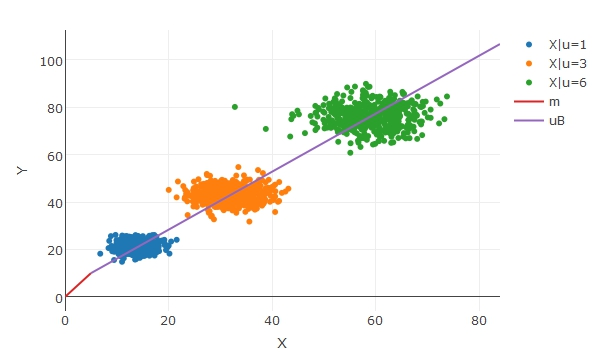
\includegraphics[scale=0.75]{Figuras/bm}
\end{figure}


Una tabla



\begin{table}[h!]
	\centering
	\caption{Descripci\'on.}
	\label{tab:table1}
	\begin{tabular}{l|c||r}
		1 & 2 & 3\\
		\hline
		a & b & c\\
	\end{tabular}
\end{table}


\begin{table}[h!]
	\centering
	\caption{Descripci\'on...}
	\label{tab:table1}
	\begin{tabular}{ccc}
		\toprule
		Some & actual & content\\
		\midrule
		prettifies & the & content\\
		as & well & as\\
		using & the & booktabs package\\
		\bottomrule
	\end{tabular}
\end{table}


Y algoritmos

%\begin{algorithm}[H]
%	\SetAlgoLined
%	\KwResult{Write here the result }
%	initialization\;
%	\While{While condition}{
%		instructions\;
%		\eIf{condition}{
%			instructions1\;
%			instructions2\;
%		}{
%		instructions3\;
%	}
%}
%\caption{How to write algorithms}
%\end{algorithm}

